\documentclass[preprint,9pt]{sigplanconf}
\usepackage{url}
\usepackage{listings}
\usepackage{subfigure}
\usepackage{times}
\usepackage{multirow}
\usepackage{color}
\usepackage{multicol}
\usepackage{amsmath}
\usepackage{amssymb}
\usepackage{setspace}
\usepackage{graphicx}
\usepackage{xspace}
\usepackage{color}
\usepackage{rotating}

\newcommand{\addtodo}[1]{\textcolor{red}{[To do: #1]}}
\newcommand{\ctrap}{CTrap\xspace}
\newcommand{\ctraps}{CTraps\xspace}
\newcommand{\ctrapsfull}{CTraps-Full\xspace}
\newcommand{\ctrapsmm}{CTraps-NRR\xspace}
\newcommand{\lws}{CTraps-LWS\xspace}
\newcommand{\lwt}{LWT\xspace}


\newcommand{\Caption}[1]{\begin{minipage}{1.0\columnwidth} \caption{#1} \end{minipage}\vspace{-2ex}}
\newcommand{\CaptionWide}[1]{\caption{#1}\vspace{-2ex}}
%\doublespacing
\authorinfo{Anonymous for Submission}{}

\title{\Large Last Writer Slices and Communication Traps}

%\authorinfo{Brandon Lucia \and Luis Ceze}{University of Washington, Department of Computer Science and Engineering}{\{blucia0a,luisceze\}@cs.washington.edu\\http://sampa.cs.washington.edu\\{\bf In Submission --- Please Do Not Distribute}}

%\author{Anonymous for Submission}
\begin{document}
\maketitle

\begin{abstract}
%Monitoring inter-thread memory dependences in production is useful.  Doing so
%improves debugging information and provides information to dynamic analyses and
%runtime systems.  Prior work that continuously monitors cross-thread
%dependences typically has overheads too high for production.  

We design efficient system support for collecting {\em last writer slices} for
shared-memory concurrent programs.  Last writer slices dynamically track memory
updates.  Last writer slices reflect the provenance of values in memory,
information that is useful during debugging.   Using last writer slices,
we build {\em communication traps} (\ctraps).  \ctraps is a mechanism that
efficiently monitors and can interpose on memory operations that share data
between threads.  \ctraps is an extensible framework, exposing
inter-thread dependences to {\em \ctraps applications} that can implement
arbitrary dependence analyses.  

We implement last writer slicing and \ctraps.  We show that last writer slices
provide information that is useful for debugging several real-world bugs.  We
show \ctraps is useful by implementing two concurrency analyses from prior
work.  We evaluate our designs on a set of server programs and standard
benchmarks.  Our results show that collecting last writer slices has low run
time overheads (0--15\%) for many important applications, like memcached,
LevelDB, MySQL, and Apache.  We show that \ctraps imposes low run time
overheads by default and that the overheads scale with the complexity of the
analysis being implemented.

\end{abstract}

\section{Introduction}
Multi-threaded programming is challenging.  In contrast to the simplicity of
sequential reasoning, multi-threaded programs require complex reasoning about
many threads of control and their interactions.  In shared memory programs,
threads interact by reading and writing memory locations.  Threads' reads and
writes interleave arbitrarily and nondeterministically and each interleaving
can yield different behavior.  Reasoning about thread interactions is a central
challenge to building multi-threaded software because some thread interactions
have undesirable consequences, like causing a crash or degrading performance.

A common approach to this challenge is to reason about dependent memory
operations.  Memory operations are dependent if their order determines the
values they read or write.  The utility of dependence information is made
especially clear by its prevalent use during manual program debugging and in
support of program analysis tools.

Debugging a concurrent program requires understanding how threads interact and
dependence information furnishes that understanding.  Dependence information
helps programmers with the difficult task of reasoning about the {\em
provenance} of a memory location's value -- control- and data-flows that
influenced that value.  Programmers debug programs more effectively when they
have access to a value's provenance at points during a program's
execution~\cite{tipslicingsurvey,whylineicse}.  In concurrent programs, data
provenance information is particularly valuable because data may originate from
any of a potentially large number of threads, making reasoning without explicit
provenance information complex and difficult.

Compounding this complexity, many concurrency bugs manifest as failures rarely.
When a deployed system fails and a programmer receives a bug report,
reproducing the reported failure to collect provenance information may be
difficult or impossible.  It is essential to collect as much information as
performance margins permit from deployed systems, to reduce the need for
time-consuming failure reproduction.  Unfortunately, prior approaches to
tracking dependences in concurrent code~\cite{raceslicing,tipslicingsurvey}
impose high run time overheads.  These overheads are prohibitively high for use
in production. 



%\cite{defuse,conseq,recon,bugaboo,raceslicing,fasttrack,falcon}
%\cite{oshajava,osha} 
%\cite{avio,dmtracker,cci,daikon}
%\cite{aviso,cfix} 
%\cite{mtperf,criticalitypredictors,schedpredictionmodel}  
%\cite{defuse}
%\cite{avio,cci,defuse,recon,bugaboo,falcon,dmtracker,aviso,cfix,criticalitypredictors,schedpredictionmodel}

Dependence information is also an important part of many program analysis
tools.    Bug detection~\cite{avio,fasttrack,raceslicing,dmtracker} and
debugging~\cite{tipslicingsurvey,bugaboo,recon,cci,defuse,conseq,falcon} tools
analyze inter-thread dependences to find buggy behavior and help programmers
understand their errors.
Profilers~\cite{threadclustering,schedpredictionmodel} analyze inter-thread
dependences to find optimization opportunities.  Dependences are also essential
to some program understanding systems~\cite{oshatr} and dynamic checkers for
thread interaction properties~\cite{oshajava,velodrome}.
Record-Replay~\cite{chimera,doubleplay,fdr,rtr} systems track and record the
order of dependent events to help reproduce failures.  These systems would be
even more valuable, if their underlying dependence analysis was run in
production.  However, the heavy-weight analyses proposed by many of these
systems impose overheads too high for production use (5-100x
slowdown)~\cite{raceslicing,dmtracker,velodrome,recon,defuse,oshajava,chimera,coredet,stm}.

%Deterministic execution
%systems~\cite{coredet,grace} monitor dependences to determine how and when to
%serialize portions of threads' executions to enforce determinism.  Software
%trasactional memory (STM) systems~\cite{stm} monitor dependences to identify
%conflicts between concurrently executing atomic code regions.  

Our goal in this work is to collect, with deployable efficiency, useful
dependence information that captures data provenance for use in debugging and
serves as a foundation for more sophisticated program analyses.  We start from
two simple observations: (1) Reads are frequent so we must minimize tracking
overheads on reads, and (2) In concurrency analyses, {\em inter-thread}
dependences are most important.  Based on these observations, we focus first on
tracking write-after-write dependences (WAWs), which provide a useful form of
data provenance information.  Building on that, we describe support for
tracking {\em communication dependences}.  Communication occurs when a thread
reads or overwrites a memory location that was most recently written by a
different thread; {\em i.e.}, inter-thread read-after-write dependences (RAWs)
as well as WAWs.  In this work, we demonstrate that this form of light-weight
dependence tracking is useful and versatile, and has inherent overheads that
are low enough for use in deployed systems.  There are two parts to our work:

First, we describe {\em last writer slices}
(Section~\ref{sec:lastwriterslices}).  Last writer slices record the thread and
program point that last wrote each memory location.     Last writer slices are
useful because they expose the provenance of a memory location's contents
during debugging (Section~\ref{sec:debugging}).  When a failure occurs, last
writer slices are saved with a core dump.  Last writer slices are also
available during an execution in the debugger ({\em e.g.}, at breakpoints).
Note that while prior work ({\em e.g.},
~\cite{recon,fasttrack,conmem,conseq,cci}) has relied on {\em ad hoc}
last-writer analyses, in this work, we isolate the essential last-writer
information in the form of last writer slices and provide an implementation
with overheads appropriate for production systems.  Tracking last writer slices
has low overhead because it imposes overhead on only write operations:  reads
are overhead-free.  In Section~\ref{sec:eval} we experimentally show that
collecting last writer slices indeed has overheads suitable for production
systems for a variety of applications.

Second, on top of last writer slices we build {\em Communication Traps} or {\em
\ctraps}  (Section~\ref{sec:ctraps}).  \ctraps monitors inter-thread
communication with overhead low enough for production use in many important
cases.  When threads communicate, \ctraps delivers a software {\em trap} that
can be handled by a trap handler.  Trap handlers implement {\em \ctraps
applications} through an extensible interface that can analyze or interpose on
the execution (Section~\ref{sec:apps}).  By default, \ctraps has very low
overhead.  \ctraps applications can perform arbitrary dependence analyses, but
at their own discretion and cost.  As we show in our evaluation, the overhead
of \ctraps applications scales with the complexity of their analysis.

\paragraph{Contributions of This Work}
To summarize, this work makes several contributions:
\begin{itemize}

\item{We describe last writer slicing, a dynamic analysis that tracks
memory updates, capturing data provenance information.  We
design and implement system support for collecting last writer slices.  }

\item{Building on last writer slicing, we describe and implement \ctraps, which
exposes inter-thread communication through an extensible trap interface.  }

\item{We evaluate the utility of last writer slices and \ctraps. We first
present several case studies that show that last writer slices are useful for
debugging real-world bugs.  We then show how \ctraps is useful for building
dependence analyses by implementing two analyses from prior
work~\cite{cci,defuse,recon}. }

\item{We evaluate our system's performance using a variety of important
applications ({\em e.g.}, MySQL, memcached and the PARSEC
benchmarks~\cite{parsec}).  We show that in many cases our designs have
overheads low enough for use in deployment (0--15\%).}

\end{itemize}




%In this work, we begin by showing that the cost of monitoring communication has
%been overstated in prior work.  We do so by designing support to monitor
%communication that, for a variety of important applications ({\em
%e.g.},databases, key-value stores, web servers) the overheads are extremely low
%-- so low that communication tracking is viable even for today's deployed
%systems.  We illustrate our claim with system support for  {\em Communication
%Traps} or \ctraps.  Our support for \ctraps tracks communication between
%threads and exposes communication events to trap handlers that can implement
%applications, such as the above.  We show the feasibility of our approach by
%implementing a selection of the above applications, as well as several novel
%applications.  We study the performance characteristics of \ctraps and provide
%a comparison to prior work, showing that our system has lower performance
%overheads -- in some cases, by one to two orders of magnitude lower.  We then
%show that even in cases that, for \ctraps, incur higher performance overheads,
%judicious use of sampling reduces overheads to an acceptable level, and retains
%many of the benefits of non-sampling \ctraps.


\section{Background}

In this section we discuss debugging with data dependence information, using an
example, in order to motivate collecting last writer slices in deployed
systems.  We then provide context for \ctraps by discussing some more
sophisticated concurrency analyses that rely on the kind of dependence
information we are focusing on in this work.

%Many systems that support programming and execution models, debugging tools,
%and other software engineering tools track dynamic memory dependences during a
%program's execution.  

\subsection{Debugging and Data Provenance}

Data provenance information is directly useful during program debugging.
Work on debugging~\cite{whylinechi,whylineicse} in the HCI and Software
Engineering community shows that when programmers debug programs, they benefit
from the ability to directly ask such provenance (``why'') questions of their
debugger.  


\begin{figure}[h]
\centering
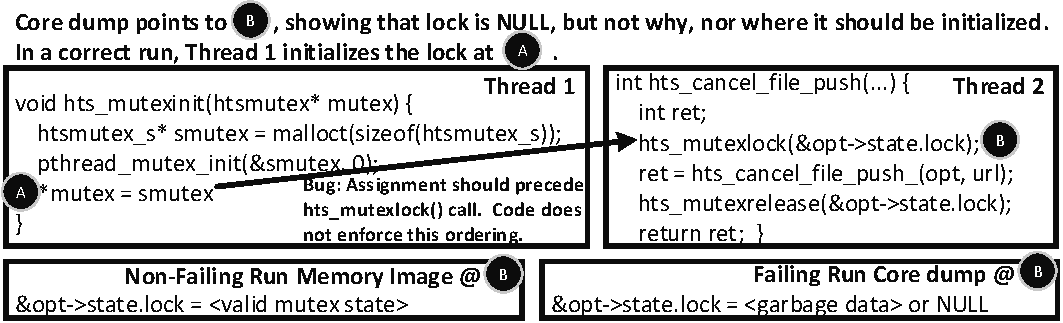
\includegraphics[width=\columnwidth]{figs/BackgroundCoreDumpFail.pdf}
\caption{\label{fig:coreDumpFail}{\bf Ordering violation bug in HTTrack.} Simply examining memory does not provide provenance information that helps understand this bug.}
\end{figure}

Figure~\ref{fig:coreDumpFail} illustrates the role that provenance information
plays in debugging, using an example of a real bug from HTTrack, a web caching
tool.  The figure depicts two threads manipulating a data structure that
contains a mutex\_lock.  The program has an ordering violation bug: the
program crashes when Thread 2 tries to acquire the lock before Thread 1 has
initialized it.  Assuming the run time environment supports it, a core dump
delivered to the programmer after such a failure reveals very little about how
to fix the bug.  The lock is uninitizalized, so the core dump may show that it
holds {\tt NULL} or it may hold random bits.  Both scenarios provide no
insight into the root cause of the failure, which is that the code permits a
use of the lock before its initialization.   Comparing the core dump from the
failing run to the memory image from a correct execution -- a helpful debugging
strategy -- reveals only that in a correct execution, the lock contains valid
mutex state.  This revalation is of limited use as it does not rule out
arbitrary data corruption as the bug's root cause.

The vital, missing piece to solving this bug is provenance information.
Debugging would be easier if the core dump included information about the
thread and code point that last wrote the lock.  The programmer would see that
no thread had initialized the lock in the failing execution, but that Thread 1
initialized the lock in non-failing executions.  This information guides the
programmer to fix the bug by adding synchronization that ensures the correct
operation ordering.

Another challenge in debugging this bug is that it manifests as a failure
infrequently and under only real-world conditions.  If the programmer runs the
program in a debugger, the failure may not manifest in a reasonable amount of
time and running it may require unavailable real-world inputs.  Thus,
collecting provenance or other information offline is time-consuming or
impossible.  A better strategy is to continuously collect that information in
deployed systems and package it with core dumps sent to programmers with bug
reports.  In this work, we propose a last writer slicing design that espouses
this {\em in situ} data collection strategy and does so with overheads
appropriate for production systems.

%Dynamic dependence slices are especially useful for debugging if they are
%available after a failure has occurred in a deployed system. However, slicing
%in deployed systems is uncommon, because deployed systems demand low overheads
%and slicing can have high overhead.  Our system provides provenance information
%that is useful at debugging time by collecting {\em last writer slices} that
%help understand inter-thread communication.  We track last writer slices with
%overhead low enough for use in production code.  Deployable efficiency makes it
%possible to collect and report last writer slices the same way today's systems
%collect and report core dumps.

\subsection{Tracking Dependences and Communication}
\label{sec:background:comm}
%\ctraps tracks dependences that correspond to {\em inter-thread communication}.

Monitoring inter-thread dependences is the foundation of many useful
concurrency analyses.  For example, in a software transactional memory (STM)
system~\cite{stm} dependences correspond to interference between accesses in
different threads that must be detected to rollback conflicting transactions.
Deterministic concurrent runtime systems~\cite{coredet,grace} are similar --
they monitor inter-thread dependences, to determine when to apply
deterministic ordering constraints on threads' accesses.  STMs and
deterministic systems must track all dependences and they must track them
precisely, to provide strong guarantees as programming and execution models.
Unfortunately, precision has a high runtime overhead -- {\em e.g.},
CoreDet incurs a mean overhead of around 5x~\cite{coredet}.  This overhead is
too high for use in production.  

%The overhead comes from the need to precisely track read-after-write (RAW),
%write-after-read (WAR), and write-after-write (WAW) dependences, taking action
%({\em e.g.}, buffering) on most cross-thread dependences.  These systems track
%dependences with additional code that runs around memory accesses.  To ensure
%correctness, accesses and tracking code usually must be protected by
%synchronization.  The high cost of synchronization exacerbates the overheads.

In contrast to {\em imprecision intolerant} tasks like STM and deterministic
execution, other tasks are more {\em imprecision tolerant}.  Imprecision
tolerant systems help perform tasks like
debugging~\cite{defuse,conseq,recon,bugaboo,raceslicing,fasttrack,falcon},
software engineering~\cite{oshajava,oshatr}, anomaly
detection~\cite{avio,dmtracker,cci,daikon}, bug and failure
avoidance~\cite{aviso,cfix} and concurrent performance
profiling~\cite{threadcriticality,schedpredictionmodel}.  These
systems also work by monitoring how data flows between threads.  They can
tolerate two important sources of imprecision.

First, many of these techniques track only an {\em ad hoc} subset of
dependences.  For example, DefUse~\cite{defuse} tracks inter-thread WAR
dependences, but not WAW dependences.  Recon tracks some inter-thread WAW and
RAW dependences and approximates WAR dependences.  These techniques are useful
despite an incomplete set of dependences.  Second, many of these systems rely
on statistical models of software
behavior~\cite{avio,cci,defuse,recon,bugaboo,falcon,dmtracker,aviso,threadcriticality,schedpredictionmodel}.
Models often tolerate noise, so many of these techniques can relax the
correctness constraints of their implementation and remain useful.  For
example, some systems have chosen not to enforce atomicity of each memory
access and its dependence tracking code, compromising precision for a boost in
performance.

These tools and techniques work in a variety of environments.  A common theme
is the advantage reaped from use in a deployment environment.  Debugging tools,
profilers, and anomaly detectors benefit from seeing diverse, real-world
behavior.  Dynamic failure avoidance techniques must work in deployed systems
to be effective.  Deployment environments demand low overheads.  

The design for \ctraps that we develop in this work monitors a subset of
inter-thread dependences that correspond to inter-thread communication.
\ctraps provides enough precision to build useful analyses and runtime systems
with overhead low enough for use in production.



\section{Last Writer Slices}
\label{sec:lastwriterslices}
A last writer slice is a dynamic property of a memory location at a point in a
program's execution.   A memory location's last writer slice is a record
containing the program point and the identifier of the thread that last wrote
data to that memory location.  We gather last writer slices at runtime by
maintaining a {\em last writer table} (\lwt) that maps from a memory
location's address to its last writer slice.  Just before a thread writes to a
memory location,  the thread first finds the memory location's entry in the
\lwt and updates that entry with its thread identifier and its current point in the
program.  After updating the \lwt, the thread performs the original memory
access.

Figure~\ref{fig:basicLWT} shows the basic operation of the \lwt.  The right
side of the figure shows a program execution with three threads.  On the left
is the \lwt at the point of each memory access.  There are two key things to
notice.  First, write operations update the \lwt entry of the memory location
they access.  Second, there is no action necessary for read operations.
Making read operations cheap is key to making the overhead of last writer
slicing low enough for deployment use.

\begin{figure}[h]
\centering
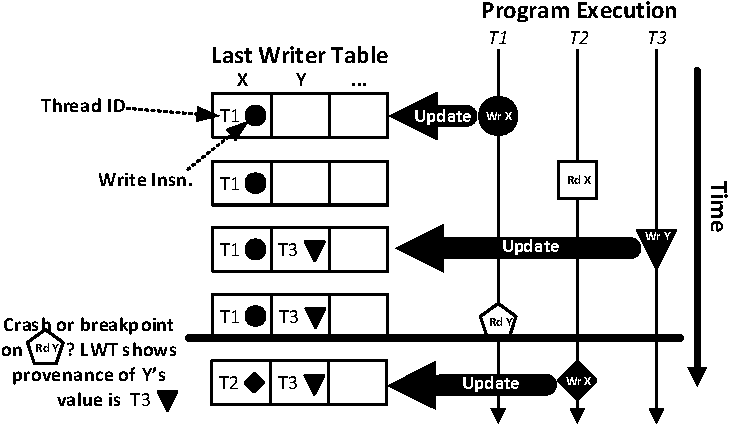
\includegraphics[scale=.6]{figs/BasicLWT.pdf}
\caption{\label{fig:basicLWT}Basic operation of the last writer table. Different shapes signify different distinct memory operations. }
\end{figure}


\subsection{Debugging with Last Writer Slices}
\label{sec:debugging}
%To answer data provenance questions during debugging, prior work has mostly
%used dependence slices that include intra-thread
%dependences~\cite{whylineicse,conseq,tipslicingsurvey}.  The overhead of
%slicing dependence chains and tracking temporal sequences is often high,
%relegating such techniques to working on traces~\cite{whylinechi} or debugging
%executions run ``in the lab''.  

At any point in an execution, the information stored in a memory location's
\lwt entry represents the provenance of the data stored in that memory
location.   Last writer slices do not explicitly record any information about
read operations and they do not need to to be useful.  Interrupting the
execution while debugging and examining an entry in the \lwt reveals the
provenance of a value just when it is needed.  For example, if an assertion
failure occurs due to an erroneous inter-thread data flow, the provenance of
the data in the assertion's condition helps explain why the failure occurred.
Computing last writer slices is fast enough to deploy and use continuously
(see Section~\ref{sec:eval}) and the \lwt can be saved with a core dump.
Thus, last writer slices can be made part of the standard debugging
information provided when a program fails.  

\begin{figure}[h]
\centering
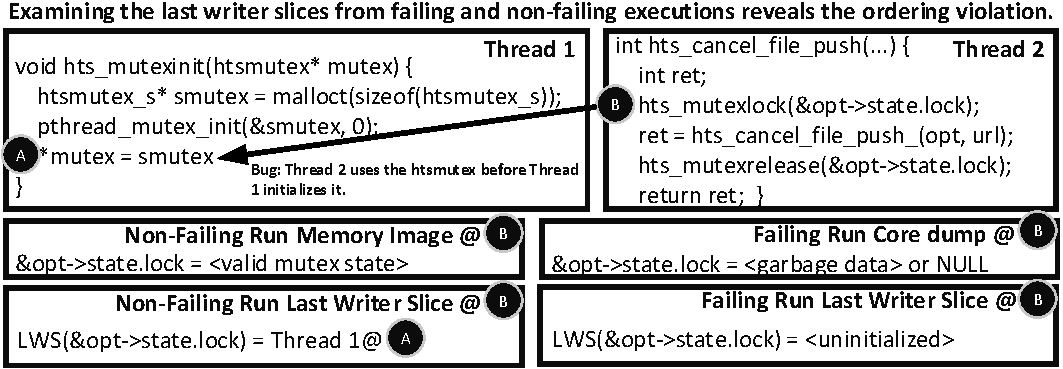
\includegraphics[width=\columnwidth]{figs/LWSHTTDebug.pdf}
\caption{\label{fig:httlws}{\bf Using last writer slices to debug an
ordering violation in HTTrack.} The provenance information stored in the last
writer slice for the mutex variable helps understand the bug's root cause.}
\end{figure}

%The core dump does not provide any
%insight into why the mutex is invalid at the time of the call or what its
%value should have been instead.


Figure~\ref{fig:httlws} shows how last writer slices help understand the root
cause of the concurrency bug from Figure~\ref{fig:coreDumpFail}.  Recall
that the the program crashes at point {\bf B} when it calls {\tt
hts\_mutex\_lock()} with an invalid mutex.    The root cause of this bug is
that Thread 1 fails to initialize the mutex before Thread 2 uses that mutex.
The last writer slices in the figure make this root cause clear: in the
failing execution, the last writer slice indicates the mutex is uninitialized; in
the non-failing execution, the last writer slice indicates the mutex was 
initialized by Thread 1 at point {\bf A}.  This information tells the
programmer that there is an ordering relationship between {\bf A} and {\bf B}
that must be enforced to fix the bug.  Note that without last writer slices,
the program crashes at {\bf B} and the core dump provides no information about
the connection between point {\bf A} and point {\bf B} -- the programmer would be left to guess that the bug was an initialization problem.

Another important trait of last writer slices illustrated by
Figure~\ref{fig:httlws} is that last writer slices are reported back to the
programmer {\em with the core dump on a failure}.  Capturing good debugging
information is especially important for concurrency bugs that manifest very
rarely or in the presence of only peculiar real-world inputs.  A primary goal
of this work is to show that we can collect last writer slices with overheads
that are low enough for production use so they can be included pervasively in
bug reports.

%We discuss last writer slices in more depth by first describing our run time
%support for collecting them.  The system support consists of a runtime library
%and a compiler analysis.  Section~\ref{sec:debugging} shows how last writer
%slices help with debugging using our running example from
%Figure~\ref{fig:bgcoredumpfail}.  We formalize last writer slices in
%Section~\ref{sec:lwssoundness}.

\subsection{Runtime \& Compiler Support}
 The \lwt is implemented as a {\em shadow memory} that holds one entry for
each memory address accessed by the program.  Each \lwt entry records the
thread and program point that last wrote to the entry's corresponding memory
location.  When a thread performs a write to a memory location, it updates the
\lwt by recording its thread identifier and the program point of its write
operation to the memory location's \lwt entry.  A program point may be an
instruction address, or a call stack.  We use instructions by default, but we experimented with 2-address bounded call-stacks as well.   

Collecting last writer slices requires instrumentation on each write operation.
We built an instrumenting compiler pass that inserts a call into our runtime
system just before each write to a memory location that may be accessed by code
executing in another thread (escaping memory accesses).  Write instrumentation
calls are passed three pieces of information: the address of the memory word
involved in the access, the thread identifier of the accessing thread, and the
accessing program point.   

\subsubsection{Escape Analysis}
We use a local function escape analysis to identify which accesses are to
memory locations that can be statically guaranteed to be inaccessible to code
running in other threads.  When a thread accesses a location that is
inaccessible to code in other threads, there is no way that access can be a
communicating access.  Such accesses are not instrumented by our compiler.  
We rely on {\tt GCC}'s built-in function escape analysis to determine if a
memory operation might lead to communication.  Locations determined not to
escape function scope also cannot escape the thread executing the function.
%Using an inter-procedural thread escape analysis may eliminate more
%instrumentation sites.  


\subsection{\lwt Formalism and Correctness}
\label{sec:lwssoundness}
To discuss the correctness of our \lwt-based last writer slice support, we
first develop a formal description of last writer slices.  We consider an
N-threaded program $P = \{P_1, P_2, \ldots P_N\}$, where $P_t = (p^{t}_{1},
p^{t}_{2}, \ldots, p^{t}_{k_{t}})$ is the sequence of $k_{t}$ dynamic
instructions executed by thread $t$.  Without loss of generality, we assume all
instructions are memory reads and writes, with the form $Op(m)$ where $Op$ is
$Read$ or $Write$ and $m$ is a uniquely addressed memory location.
A point in an execution of $P$ after $e$ instructions have
executed is defined by $Q = \{q_{0}, \ldots, q_{e}\}$ where each $q \in Q$ is a
$p^{t}_{j}$ from one of the $k_t$ instructions of thread $t$.  We introduce
$LWS[m]$ -- the Last Writer Slice for memory location $m$.   At any point $Q$,
$LWS[m]$ holds $(t,p^{t}_{\ell w})$, where $p^{t}_{\ell w} = max_{\ell}( 
q_{\ell} = Write(m) \in Q)$ and $t$ is the thread that
executed $p^{t}_{\ell w}$. Informally, $p^{t}_{\ell w}$ is the last instruction
in $Q$ to write $m$ and $t$ is the thread that executed it.  For a
never-written location $n$, $LWS[n] = (\emptyset,\emptyset)$ indicating it is
unwritten.

For our design to be correct, $LWT[m]$, the entry for a memory location $m$ in
our \lwt implementation, must be the same as $LWS[m]$ at all points in an
execution.  Correctness in the \lwt requires {\em soundness} and {\em
completeness}.  A {\em sound} design only updates $LWT[m]$ when $m$ is written.
A {\em complete} design always updates $LWT[m]$ when $m$ is written.  Our
compiler inserts \lwt updates before every write operation (for completeness)
and only before write operations (for soundness).  Formally, given a program,
$P$, our compiler pass transforms it to a new program, $P'$.  Each thread in
$P'$ executes a modified sequence of instructions: $P'_{t} \in P' = \{
I(p^{t}_{1}), p^{t}_{1}, \ldots, I(p^{t}_{k_{t}}), p^{t}_{k_{t}} \}$.
$I(p^{t}_{j})$ sets $LWT[m] = (t,p^{t}_{j})$ if and only if $p^{t}_{j} =
Write(m)$ and is a no-op otherwise.  This reasoning shows our \lwt is both
sound, complete, and thus correct.

Next we discuss two nuances of our design: (1) the interaction of our \lwt
implementation with code containing data-races; and (2) the correctness of the
\lwt when a program addresses data that overlap in memory. 

\paragraph{Consistency and Atomicity}

Our implementation of the \lwt does not add any synchronization to the program.
As a result our analysis does not incur the overheads or possible thread
schedule perturbation synchronization can cause.  However, there are two
potential issues that stem from this design choice. First, we do not enforce
memory consistency of meta-data reads and writes in different threads.  Second,
our implementation does not enforce the atomicity of \lwt updates and their
corresponding program accesses.  In the absence of data-races our \lwt
implementation is {\em always correct} and neither of these issues exist.  Both
atomicity and ordering is enforced by the program synchronization that ensures
consistency for the data being written by the instructions our system
instruments.   

We use our \lwt formalism to show that without data-races, \lwt updates and
their corresponding memory accesses are atomic and well-ordered.  The relation
$p \prec q$ denotes that $p$ happens before $q$.  In correctly synchronized
code, any write by thread $t$ to $m$, $p^{t}_{j} = Write(m)$, is ordered by
program synchronization with $p^{t'}_{j'} = Op(m)$, a later access to $m$ by
any other thread $t'$ -- {\em i.e.}, $p^{t}_{j} \prec p^{t'}_{j'}$.  Our
compiler inserts an \lwt update $I(p^{t}_{j})$ into $P'$ before its write
operation, $p^{t}_{j}$. Thus, $I(p^{t}_{j}) \prec p^{t}_{j}$ due to program
order.  Happens-before is transitive, so without data-races, $I(p^{t}_{j})
\prec p^{t}_{j} \prec I(p^{t'}_{j'}) \prec p^{t'}_{j'}$, meaning $I(p^{t}_{j})$
happens before all accesses that $p^{t}_{j}$ happens before {\em and before
their respective \lwt updates}, $I(p^{t'}_{j'})$.  Symmetrically, for any
access $p^{t''}_{j''}$ in another thread $t''$ that precedes $p^{t}_{j}$,
$p^{t''}_{j''} \prec p^{t}_{j}$.  Our compiler inserts each $I(p^{t}_{j})$
immediately before each $p^{t}_{j}$, so $I(p^{t''}_{j''}) \prec p^{t''}_{j''}
\prec I(p^{t}_{j}) \prec p^{t}_{j}$, happens-before ordering $I(p^{t}_{j})$
after all preceding accesses to $m$ in other threads, {\em and after their
repective \lwt updates}.  Thus, at all points $Q$ in a data-race free
execution, given $q_r = I(p^{t}_{j})$, $q_p = p^{t}_{j}$, and $q_r \prec q_p$,
$\forall_{ \{q_s | q_r \prec q_s \prec q_p \}}: q_s \ne Op(m) \wedge q_s \ne
I(Op(m)) $.  In other words, \lwt updates and their accesses are atomic.

In a program with a data-race, there are some accesses, $p^{t}_{j}$ and
$p^{t'}_{j'}$, that are concurrent.  The \lwt updates for these accesses are
also concurrent because they are not transitively ordered by the accesses' ordering.  The unordered accesses and \lwt updates can interleave arbitrarily
because they are concurrent.  Some racy thread schedules may violate the
atomicity of accesses and their \lwt updates.  Such an execution could reach a
state $Q_{bad} = (\ldots, I(p^{t}_{j}), I(p^{t'}_{j'}), p^{t'}_{j'}, p^{t}_{j},
\ldots)$ and in that state, $LWS[m] = (t,p^{t}_{j})$, but $LWT[m] =
(t',p^{t'}_{j'})$.  The \lwt was effectively not updated when $p^{t}_{j}$
executed (violating completeness), or was effectively updated to reflect that
$p^{t'}_{j'}$ was $m$'s last writer, when $p^{t}_{j}$ was (violating
soundness).    

According to the C++11 language specification, in the presence of a data-race,
a program's behavior is undefined and arbitrary state corruption can occur.  In
the presence of data-races, {\em any} analysis, including our \lwt analysis,
running on such a program could experience arbitrary corruption.  In practice
({\em e.g.}, on x86) these atomicity violations may cause limited \lwt
corruption, but even this is unlikely.  These atomicity violations only occur
only when accesses to the same data occur within a very short time interval,
which is uncommon, {\em and} an unserializable interleaving of accesses and
\lwt updates also occurs.

{\bf TODO: Figure?}




\paragraph{Non-overlapping Memory References} 
We assume each written memory location corresponds to a non-overlapping memory
region because our \lwt design is {\em granularity oblivious}.  We discuss this
issue informally due to space constraints.  Each \lwt entry corresponds to a
memory location referenced by a program instruction.  Two instructions might
reference different locations that overlap because the referenced locations
have different granularities ({\em e.g.}, accessing a byte that is part of a
previously accessed word).  When that happens, both accesses update different
\lwt entries, because they reference different locations.  However, the
overlapping region then has two different entries reflecting the last {\em two}
updates to its parts rather than just its last write.

The \lwt remains correct, assuming the program only accesses non-overlapping
regions.  In programs that access overlapping regions, there is always some
entry in the \lwt that correctly reflects each memory location's last writer.
However, the entry for a coarse-grained region may be obsolete because of an
access to an overlapping sub-region.

One approach to mitigating this issue would be to allocate \lwt entries for
regions of fixed granularity.  We chose not to do so for two reasons.  First,
associating \lwt entries with regions of  large granularity only ({\em i.e.},
cache-line) precludes sound analysis for fine-grained accesses.  Second,
associating \lwt entries with regions of small granularity ({\em i.e.}, byte)
requires multiple \lwt updates for larger granularity accesses, increasing
their overheads proportionately to the granularity of the access.





\section{Communication Traps}
\label{sec:ctraps}

\ctraps is a framework for analyzing and interposing on inter-thread
communication events during a program's execution.  We build \ctraps on top of
last writer slicing that we described in Section~\ref{sec:lastwriterslices}.
Using last writer slice information, \ctraps dynamically tracks 
inter-thread communication events. \ctraps exposes communication
events as {\em traps} during an execution that {\em trap handlers} can handle
to perform analysis and interposition.  We formalize trap delivery and handling
in Section~\ref{sec:ctsoundness}.

\subsection{\ctraps Design}

We now discuss \ctraps in more detail by describing the design of our \ctraps
system support.  Figure~\ref{fig:systemdiagram} shows an overview of our system
support.  The programmer writes their program as usual.  They compile it using
the \ctraps compiler. The \ctraps compiler includes the compiler support for
collecting last writer slices.  In addition, the \ctraps compiler also inserts
calls to the \ctraps runtime at points where communication may occur.  The
resulting compiled executable links to the \ctraps runtime that collects last
writer slices and monitors communication.  The runtime loads and manages \ctraps
handlers when the execution starts via a plugin interface.  \ctraps handlers,
written independently of the original program implement \ctraps applications.
Traps are delivered to handlers by the runtime when operations communicate.
Together, the \ctraps executable and the \ctraps handlers are deployed.


\begin{figure}[htb]
\centering
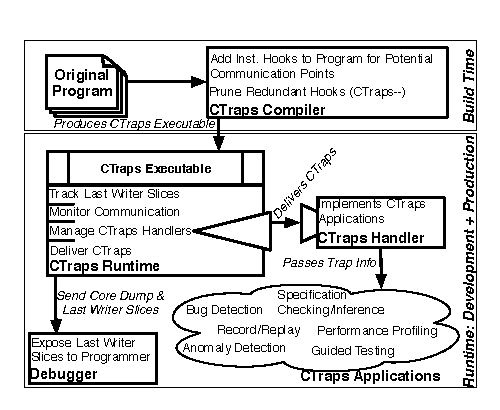
\includegraphics[width=.90\columnwidth]{figs/SystemDiagram.pdf}
\caption{\label{fig:systemdiagram}CTraps system support.}
\end{figure}


%Our system support for \ctraps incorporates the support for collecting last
%writer slices described in Section~\ref{sec:lastwriterslices}.  In addition,
%our \ctraps system support also monitors all read and write operations that
%might communicate and traps on all those that communicate.  

\subsubsection{Compiler and Runtime Support} 

\ctraps delivers software traps before all read and write operations executed
by one thread that access a memory location that was last written by another
thread, {\em i.e.}, communicating memory operations.  Traps are simply function
calls made before such operations execution.  \ctraps implements traps using a
combination of compiler and runtime library support.

\paragraph{Compiler Support}
Our compiler inserts a call to the \ctraps {\em trap hook} function immediately
before all read and write operations that access potentially escaping memory
locations.  Trap hooks are passed the address of the memory location being
accessed, the thread identifier of the accessing thread, the type of operation
being performed, and the program point of the access.  

\paragraph{Runtime Support}
The \ctraps runtime implements the trap hook function,  which has two purposes.
The trap hook function detects communication and delivers traps to \ctraps
applications when communication occurs.  The trap hook function detects
communication by looking up the \lwt entry for the memory location being
accessed.  If the thread identifier in the \lwt entry is different from the
accessing thread, then the trap hook function delivers a trap to the accessing
thread, just before the memory access is allowed to proceed.  To deliver a
trap, the trap hook function calls {\em trap handler routines} that are defined
in \ctraps applications.  Trap handler routines are like signal handlers.  They
are registered with the \ctraps runtime when the program starts.  Trap handlers
may contain arbitrary application-specific code.  Figure~\ref{fig:hookapi}
shows the \ctraps trap handling API.  Trap handlers are passed the four pieces
of information passed to the trap hook, as well as the \lwt's record of the
program point and thread identifier of the last write to the involved memory
location.

\begin{figure}[htb]
\centering
\begin{verbatim}
void trap(AccessType type, 
          ThdId currThd, ProgPt currPt,
          ThdId lastThd, ProgPt lastPt);
\end{verbatim}
\caption{\label{fig:hookapi}The \ctraps trap handling interface.}
\end{figure}

\subsection{Formalism and Correctness}
\label{sec:ctsoundness}
To discuss the correctness of \ctraps, we first formalize trap delivery by
building on our last writer slicing formalism from
Section~\ref{sec:lastwriterslices}.  

Given a program $P'$ already instrumented with \lwt updates, the \ctraps
compiler produces $P''$. A thread $t$ in $P''$ executes a modified instruction
sequence, $P''_{t} = \{ T(p^{t}_{j}), I(p^{t}_{1}), p^{t}_{1},$ $\ldots,
T(p^{t}_{j}), I(p^{t}_{k_{t}}), p^{t}_{k_{t}} \}$, where $T(p^{t}_{j})$ is a
trap hook call.  We consider a point $Q = \{q_1, \ldots, q_{e-2}\}$ after $e-2$
instructions of an execution have executed and $q_{e} = p^{t}_{j}$ is about to
execute after its trap hook $T(p^{t}_{j})$ and \lwt update $I(p^{t}_{j})$
execute.  The trap hook $T(p^{t}_{j})$ {\em delivers} a trap before if $LWT[m]
= (t',p^{t'}_{\ell w})$ and $t \ne t'$.  Informally, the trap hook delivers a
trap before the instruction if the thread that last wrote $m$ is different from
the one executing the instruction.  When a trap hook, $T(p^{t}_{j})$, delivers
a trap, thread $t$ executes an arbitrary trap handler $H = \{h^{t}_{1}, \ldots,
h^{t}_{h_{n}}\}$.  Thus, after the trap, the \lwt update, and the instruction
execute, the execution reaches the new point $Q = (q_{1}, \ldots, T(q_{e}),
h^{t}_{1}, \ldots, h^{t}_{h_{n}}, I(q_{e}), q_{e})$, and continues.

A \ctraps implementation must be sound and complete to be correct.  A design is
{\em sound} if it only delivers a trap when threads have communicated.  A
design is {\em complete} if it always delivers a trap when threads have
communicated.  The \ctraps compiler puts a trap hook on all read and write
operations, and only on those operations.  Assuming a correct \lwt, \ctraps is
correct.  Our \ctraps implementation also does not insert any synchronization
into the program, so it comes with the same caveats related to data-race
freedom as the \lwt.  The same arguments for \lwt correctness apply to the
correctness of trap delivery and handling.  Most importantly, data-race freedom
implies that trap hooks, \lwt updates, and accesses are all atomic.


%\paragraph{Escape Analysis}
%All our designs eliminate instrumentation on accesses to memory locations
%statically guaranteed to be inaccessible to other threads.  Doing so has no
%effect on soundness or completeness because accesses to such locations are
%guaranteed never to be communicating.


\subsection{\ctraps Applications}
\label{sec:apps}
\ctraps applications are implemented as shared library plugins that are loaded
by our runtime.  They must implement the \ctraps trap handler API, which
requires a trap handler function and permits a constructor, destructor, thread
constructor, and thread destructor, which allow initialization and disposal of
global and thread-local state.  Many useful \ctraps applications are possible,
several of which were outlined in Section~\ref{sec:background:comm}.    To
demonstrate that \ctraps can implement real analyses with little work, we
implemented two applications. The first application is a version of a debugging
analysis from CCI~\cite{cci}.  The second application is a communication graph
collector, similar to DefUse~\cite{defuse}, Recon~\cite{recon}, and
DMTracker~\cite{dmtracker}.

\paragraph{CCI-Prev Implementation}
CCI-Prev is a technique from CCI~\cite{cci} that records a set of code points
that access a memory location when the previous access to the same location was
by a different thread.  We implemented a variant of CCI-Prev using \ctraps that
records such a set of code points.  In our implementation, communcating read
operations update the LWT like writes normally do.  Under this policy, any
operation that accesses a location that was last accessed by a different thread
is recorded.  The set of recorded accesses is the output of the analysis.  Our
\ctraps implementation of CCI-Prev took about 10 lines of code (on top of our
base system). 

\paragraph{Communication Graph Implementation}
Communication graphs are the basis of several prior debugging
techniques~\cite{recon, bugaboo, defuse}.  We implement communication graph
collection using \ctraps.  When a trap is delivered, our implementation records
communication graph edges composed of the code point of the last writer to the
location being accessed and the code point of the trapping access.  The set of
recorded edges is the tool's output.  Our \ctraps implementation of
communication graphs took about 50 lines of code (including output formatting
code). 

\paragraph{Other Applications}
In addition to those applications, we envision that a variety of applications
will be enabled by our simple interface.  Anomaly detection and ``likely
invariant'' techniques similar to AVIO~\cite{avio}, Daikon~\cite{daikon}, and
others are a natural fit for \ctraps.  \ctraps provides the support necessary
for implementing specification checkers for specifications related to
inter-thread communication~\cite{velodrome,oshajava}.  Guided testing
tools~\cite{cuzz,chess} and bug detection tools~\cite{ctrigger} focused on
concurrency could also be implemented as \ctraps applications.  \ctraps also
provides an interesting platform for developing new approaches to
record/replay~\cite{chimera,fdr}.  \ctraps is an enabling platform for
developing these or other analyses with low baseline overheads and without the
need to build an entire concurrency analysis from scratch.

\section{System Implementation and Applications}

We implemented last writer slicing and \ctraps.  We built our compiler support
as a plugin for GCC ({\tt gcc-4.7.0 20111112}).  We used GCC's points-to and
escape analysis support to prune instrumentation to non-escaping memory
locations.  Our compiler instruments calls to {\tt free} and {\tt delete} as
writes to the pointer being deallocated.  Our analysis handles all code
compilable using this version of GCC except for a few cases: we do not handle
accesses that compile to GCC {\tt BITFIELD\_REFERENCE} IR types because these
are undocumented, we do not handle inlined assembly instructions, and we do not
handle C++ exceptions.  Note that these limitations of our research prototype
are not fundamental and the limited cases are uncommon.   

We built our runtime system from scratch in about 1000 lines of C and C++ code.
We implemented the LWT as a fixed size 2GB array of 64-bit words.  Each entry
packs a program point and a thread identifier into the 64-bit word.  By
default, program points are single instruction addresses, but we also support
limited (2-address) context-sensitivity by packing the current instruction's
address and the nearest return address into a 64-bit LWT entry. When an access
to a memory location occurs, we index into the LWT with the lower bits of the
location's address.  Our prototype implementation uses a lossy resolution
policy for hash collisions.  We use this policy in our prototype because it is
faster and simpler than a chaining concurrent hash table implementation.
Collisions are extremely rare, so this simplification is unlikely to be a
problem even in a more industrial strength implementation.  

We released our implementation, free and open-sourced~\cite{ctrapsonweb}, on
the web and have had contributions to our codebase from members of the GCC
development community.

\section{Evaluation}
\label{sec:eval}
We evaluated last writer slices and \ctraps along several axes.  We show that
last writer slices provide information that is useful during debugging in
Section~\ref{sec:eval:debugging} using case studies on several buggy programs.
We evaluate our performance overheads and show that last writer slices and
\ctraps are feasible for use in deployed systems for a majority of workloads we
studied.  We then characterize our instrumentation and discuss the sources of
our system's run time overhead.   We show that \ctraps is useful by
implementing two existing applications and analyzing their performance.    

\subsection{Debugging with Last Writer Slices}
\label{sec:eval:debugging}
We illustrate the debugging benefits of last writer slices by using our system
to debug several real-world programs studied previously in the debugging
literature.    

\paragraph{HTTrack}
The running example in Figures~\ref{fig:coreDumpFail} and ~\ref{fig:httlws},
and the text in Section~\ref{sec:debugging} describes the benefit provided by
last writer slices in debugging an ordering violation in HTTrack-3.43.9.  

\paragraph{PBZip2}
We conducted a case study using a buggy version of PBZip2-0.9.1.    The bug is
a use-after-delete bug that leads to an assertion failure.  A worker thread
tries to acquire a mutex after it has been deleted by the main thread during
shutdown, causing the assertion to fail.  

Last writer slices provide the key piece of information to debug this failure.
When the program fails, the core dump shows that the mutex is invalid because
it has been deleted.  The mutex's last writer slice shows that the last write
to the mutex before the worker tried to acquire it was when the main thread
deleted it.  The last writer slice reveals the connection between the the two
pieces of code involved in the bug: the code that acquires the mutex and the
code that deletes the mutex.  Note that this connection is not obvious when the
program crashes because the main thread may have executed arbitrarily far from
where it deleted the mutex before the worker thread crashes.  

\paragraph{MySQL}

We used last writer slices to debug an atomicity violation in MySQL-4.0.12 that
is a critical security vulnerability.  Figure~\ref{fig:mysqllws} shows the
buggy code.  Thread 1 rotates the database's log file, marking it closed,
opening a new log file, then marking it open again.  Log rotation should be
atomic, but the lack of synchronization allows Thread 2 to run its insert
during log rotation.  The insert code checks if the log is marked closed. If
the log is marked closed, the insert is not logged, manifesting the failure.
We added an {\tt abort} statement to the non-logging case because this behavior
is a security vulnerability that the bug report describes as ``critical''.
Adding this {\tt abort} is reasonable, as the bug report describes the
condition in the {\tt else} block as being an error.

\begin{figure}[h]
\centering
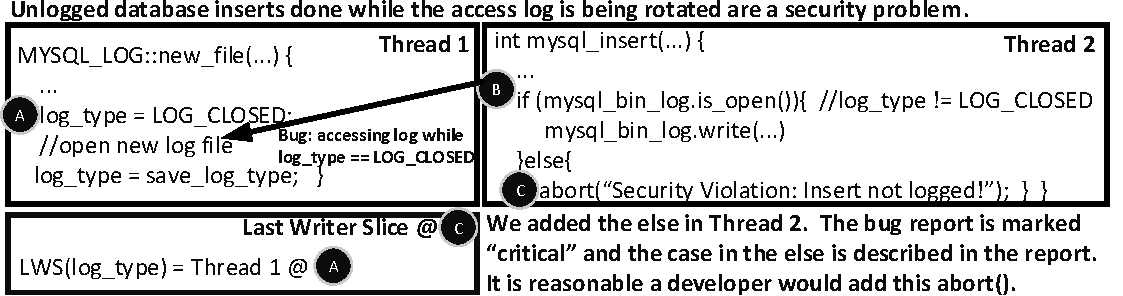
\includegraphics[width=\columnwidth]{figs/MySQLDebug.pdf}
\caption{\label{fig:mysqllws}{\bf Using last writer slices to debug an
atomicity violation in MySQL 4.0.12.} The last writer slice reveals the code that closes the log before a database insertion that goes unlogged, which is a security problem.}
\end{figure}

We triggered the bug by running an insert query during a log rotation.  The bug
manifested, stopping execution at {\bf C}.  As described in the bug report, the
query went unlogged and examining the core dump revealed the log was marked
closed at point {\bf B} ({\em e.g.}, {\tt log\_type} was {\tt LOG\_CLOSED}).
However, the core dump did not reveal {\em why} the log was marked closed
there.  The last writer slice at {\bf C} for the {\tt log\_type} variable shows
that it was written last by Thread 1 at {\bf A}.  Without the last writer
slice, the relationship between the log rotation code and the insert code is
not apparent. The last writer slice reveals that the log rotation code
interacts with the insert code incorrectly via the {\tt log\_type} variable.  


\paragraph{JDK-StringBuffer}

Last writer slices help elucidate a subtle atomicity violation in the
StringBuffer library in version 1.4 of the Java JDK.  We use the C++ port of
the buggy JDK and a driver program code developed in prior concurrency debugging
work~\cite{concurrencybugs}.  


Figure~\ref{fig:jdklws} shows how the bug can manifest as a failure. The string
object pointed to by {\tt sb} in Thread 1's code contains a string buffer and a
variable called {\tt count} that stores its length.  The {\tt append()}
code should atomically read {\tt sb->count} and update the string's buffer.
The failure occurs when the {\tt append()} code in Thread 1 is interleaved with
the {\tt erase()} code in Thread 2 as indicated in the figure.  The {\tt
erase()} code updates the buffer's length, making the version Thread 1 read
stale.  Thread 1 uses its stale version in the function called at point {\bf
B}, causing a crash.  

\begin{figure}[h]
\centering
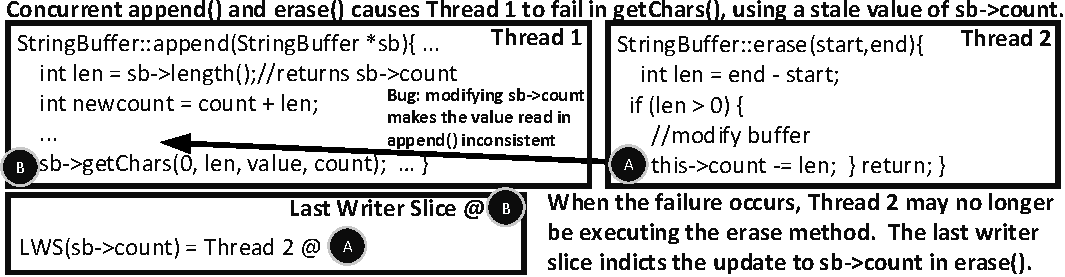
\includegraphics[width=\columnwidth]{figs/JDKStringBufferDebug.pdf}
\caption{\label{fig:jdklws}{\bf Using last writer slices to debug an
ordering violation in the JDK 1.4 StringBuffer library.} The last writer slice reveals the interaction between the erase function and the append function that leads to a failure.}
\end{figure}

When the atomicity violation manifests, the appending thread is updating the
string's underlying buffer.  The erasing thread, however, may have completed
its erase operation.  The execution context of the erasing thread at the point
of the failure provides no insight as to why the program failed.  Examining the memory image, the programmer can only conclude that the length and buffer are 
inconsistent, but not why they are inconsistent.

This situation illustrates the value of the provenenace information furnished
by last writer slices.  At the point of the failure the last writer slice for
the length variable points to a decrement of that variable in the erase
function.  The last writer slice illustrates the need for synchronization
between the append function and the erase function.  


\subsection{Performance Evaluation: Setup and Benchmarks}

We conducted our evaluation on a machine running Linux 2.6.27-7, with a 2.27GHz
8-core Xeon E5520 processor with 2-way SMT ({\em i.e.}, 16 execution contexts)
and 10GB of memory.  We evaluated our system using PARSEC, a set of
architectural benchmark programs~\cite{parsec} and a collection of real server
and desktop applications.    

\subsubsection{PARSEC}

We ran PARSEC programs with their {\tt native} input set, and with each
program's 8 thread configuration. We have omitted three of the PARSEC
benchmarks because our compiler pass does not handle C++ exceptions.    

\subsubsection{Servers}


\paragraph{MySQL-5.1.65} MySQL is an industrial-strength database
server. To benchmark MySQL, we used {\tt SysBench OLTP} running with its
default 8 threaded configuration, measuring MySQL's performance to be the
throughput reported by {\tt SysBench}.  

\paragraph{Apache-2.4.3} 
Apache-httpd is a popular web server.  To benchmark Apache, we used {\tt
ApacheBench} to request a static {\tt html} page 1,000,000 times using 8
threads, measuring Apache's performance to be the throughput reported by {\tt
ApacheBench}.  

\paragraph{LevelDB-1.5.0}
LevelDB is a carefully tuned high-performance key-value store written by Google
developers. To benchmark LevelDB, we used the included {\tt db\_bench} utility,
running its ``Read while Writing'' test with 8 threads.  We measure LevelDB's
performance to be the operation throughput reported by {\tt db\_bench}.

\paragraph{Memcached-1.4.4}
Memcached is an in-memory key-value store frequently used as a cache for web
services.  We were unable to find a standard benchmark for Memcached.  Instead,
we wrote a C program that uses libmemcached-0.49 to issue a
mixture of 10\% load requests and 90\% store requests for a single key 
simultaneously from 8 threads.  We measured Memcached's performance to be the
total time to complete 10,000 requests in each thread.


%\begin{table}
%\begin{tabular}{ l | l | c | l }
%& & & \\ \hline
%\multirow{9}{*}{\begin{sideways}PARSEC\end{sideways}} & blackscholes & & \\
%&dedup & & \\
%&canneal & & \\
%&x264& & \\
%&vips& & \\
%&ferret& & \\
%&fluidanimate& & \\
%&swaptions & & \\
%&streamcluster & & \\ \hline
%\multirow{4}{*}{\begin{sideways}Servers\end{sideways}}&MySQL & & \\
%&Apache & & \\
%&LevelDB & & \\
%&Memcached & & \\ \hline
%\multirow{3}{*}{\begin{sideways}App\end{sideways}}&PBZip2 & & \\
%&AGet & & \\
%&Transmission & & \\
%
%\end{tabular}
%\caption{\label{tab:benchmarks}\addtodo{build this table, show LOC, \#threads, sharing pattern(?), etc}}
%\end{table}


\subsection{Performance Evaluation}
\label{sec:eval:perf}

The main performance result of our work is that our designs impose performance
overheads that are low enough for use in deployed systems for many of our
experimental workloads.  Figure~\ref{fig:perfall} shows the slowdown suffered
by our benchmarks due to last writer slicing and \ctraps running with ``no-op''
trap hooks ({\em i.e.}, no handlers), relative to the natively executing
baseline.  These data reflect our main performance findings.    

\paragraph{Last Writer Slices}
The data show that last writer slicing has very low overheads with a geometric
mean of less than 10\% across our server programs and less than 50\% across
PARSEC.  Such low overheads are very likely to be tolerable in deployed
systems.  In many cases (Apache, MySQL, {\tt dedup}, {\tt canneal}), overheads
are negligible.  In all but two cases ({\tt vips} \& {\tt swaptions}), the
overhead of collecting last writer slices is less than 100\%.    

\paragraph{\ctraps}
\ctraps imposes a geometric mean overhead of 14\% for server applications
and 110\% for PARSEC applications.  In 7 out of 13 of our tests, the overhead
of \ctraps is less than 50\%.  These seven low overhead benchmarks include
all of our server programs, as well as {\tt blackscholes}, {\tt dedup} and {\tt
canneal} from PARSEC.  The overhead for these applications is likely to be
tolerable in production.  {\tt vips} and {\tt swaptions} saw the highest
overheads -- around 400\%.  We discuss sources of high overheads in
Sections~\ref{sec:eval:conservative} and~\ref{sec:eval:parsecserver}.

By comparing \ctraps and last writer slicing, we see four applications ({\tt
dedup}, {\tt streamcluster}, {\tt fluidanimate}, {\tt ferret}) that have
\ctraps overhead that is probably too high for always-on use (averaging 153\%)
drop to a last writer slicing overhead that is probably low enough for always-on use
(averaging 38\%).  The large decrease indicates these programs perform
relatively more reads than other applications, and thus benefit more from
eliminating read instrumentation.
%\paragraph{\ctrapsmm}
%\ctrapsmm has very similar overheads to \ctrapsfull in most cases.   The only case
%with a major difference was {\tt vips}, indicating it executes more redundant
%reads than the other applications.  The similarity in the two designs'
%overheads is expected because our default ``no-op'' read instrumentation does
%not contribute much to overheads in most cases.  Hence, unless \ctrapsmm culls
%calls with high dynamic frequency, it is unlikely to reduce overheads much.  We
%show in Section~\ref{sec:appperf} that \ctrapsmm provides more performance
%benefit when used to implement applications that make read instrumentation sites
%more costly.
\\
\\
These high-level results support our main claim that the runtime overhead of
\ctraps is low enough for deployed systems for many 
applications, especially for servers.  We now further analyze our observed overheads, illuminating
differences between the lower-overhead server programs and the higher-overhead
PARSEC programs.

\begin{figure}
\centering
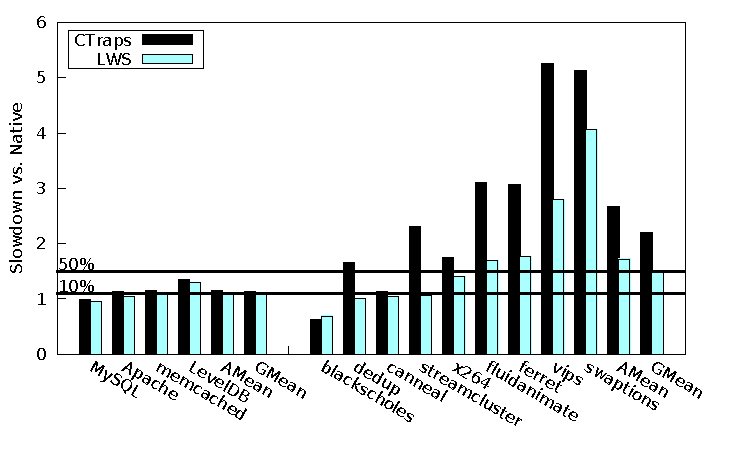
\includegraphics[width=.9\columnwidth]{plots/perf.pdf}
\caption{\label{fig:perfall}Runtime overhead of \ctraps and Last Writer Slices (LWS).}
\end{figure}

\subsubsection{Overheads Due to Conservative Escape Analysis}
\label{sec:eval:conservative}
{\tt swaptions} had the highest overheads in our tests.  We investigated their
cause and determined they are mostly artificial and due to shortcomings of our
escape analysis.  We located the inner-loop function {\tt
HJM\_SimPath\_Forward\_Blocking}.  The function uses two local matrices that
are allocated through an external call.  Our escape analysis cannot determine
that the call only does allocation and that the matrices are local, so it
conservatively assumes the matrices escape.  We manually inlined the allocation
(and a matching deallocation), and escape analysis eliminated their
instrumentation.  The program's overhead dropped from about 420\% overhead for
\ctraps to about 300\% overhead; the change for last writer slicing was from 300\% to about
130\% overhead.  We also looked at an output matrix passed into the inner-loop
function.  The matrix is allocated and deallocated in the inner-loop's caller,
but is never shared.  Eliminating instrumentation on accesses to this matrix
yielded an overhead of about 46\% for \ctraps, and to just 30\% for
last writer slicing.

Note that both these changes amount to inlining and preserve the semantics and
sharing pattern of the program.  We expect that more sophisticated escape
analysis would find these local accesses and achieve these performance gains
automatically.


\subsubsection{PARSEC vs. Servers}
\label{sec:eval:parsecserver}
In our tests, server programs were better able to tolerate the overhead of
last writer slicing and \ctraps.   We discern three reasons for this difference.

\paragraph{Independent Parallelism}
In most cases, servers have more independent parallel work.  Server programs
set up a pool of threads to handle requests.  Each thread incurs some
instrumentation latency, but that latency is hidden by other threads making
progress on independent requests.  This analysis also applies to the PARSEC
applications that had performance similar to the servers.  For instance, {\tt
blackscholes} uses largely independent threads to compute on different regions
of a matrix.  In addition, threads performing independent computation ({\em
i.e.}, non-communicating computation) are likely to operate mostly on
non-escaping, local data.  Local data are not instrumented by our compiler,
sparing the overhead.  We characterize the amount of local data in each
application in detail in Section~\ref{sec:char}.  We show that the server
programs have a larger proportion of provably local accesses than PARSEC.  The
difference supports the fact that the servers have more independent work ({\em
i.e.}, more local accesses) than PARSEC. 



\paragraph{Latency Hiding I/O}
The servers perform more I/O.  Similarly to the effect of abundant parallelism,
I/O helps hide instrumentation latency.  While I/O is naturally part of many
applications, we aimed to minimize the effect of I/O in our experiments.  For
MySQL and Apache, we used local disks for logs and resources, and connected via
a local socket, rather than using the network.  In spite of these controls, I/O
remains, and hides latency in our server applications.  LevelDB's benchmark is
designed to avoid all I/O, creating and manipulating a database entirely in a
single process.  The absence of I/O may account for some of the difference in
overhead between LevelDB and the other servers.  Note that the effects of I/O
are not merely experimental noise -- in real deployed software the latency
hiding effects of I/O are likely to be even {\em more} pronounced.


\paragraph{Interference with Optimization}
The PARSEC programs are more heavily hand-optimized. In several cases
resorting to hand-coded assembly and cache-aware memory access patterns.
Running instrumentation that accesses the \lwt alongside these computations may
disrupt their cache performance, or other delicately optimized behavior,
leading to higher overheads.  

Such carefully optimized code is likely to have been written by expert
programmers.  As with other code written by experts ({\em e.g.}, lock-free
data-structures), this code may not require as much {\em in situ} analysis
support as code written by distributed teams of open source developers or
novice programmers.  Depending on the maturity and level of verification of a
piece of carefully hand-optimized code, it might make sense to elide all
communication tracking instrumentation to preserve performance. 
 

%\subsubsection{Breaking Down the Design Space}
%Figure~\ref{fig:perfall} also shows the impact of context-sensitivity, lossy
%optimization, and sampling on our overheads.  
%
%\paragraph{Context Sensitivity}
%Context-sensitivity imposes a substantial overhead in some cases.  The
%additional cost of context-sensitivity is about 10\% of the total overhead for
%PARSEC.  For server applications, the cost is less substantial, but still a
%non-negligible 4\% over the baseline.  The cost of context-sensitivity comes
%from the need to compute and store multiple addresses, rather than a single
%program counter.  
%
%In the context insensitive case, updating the \lwt requires a single register
%read ({\em rip}) a bitwise {\tt or} to combine the thread identifier and the
%instruction pointer, and the actual write to update the \lwt entry.  In the
%context sensitive case, updating the \lwt requires looking back over the call
%stack, and a bitwise {\tt or} operation at each return address.  The cost is at
%least a multiple of the cost of the constext insensitive case.  However, to
%restrict overhead to write instrumentation calls, we walk stack frames, rather
%than iteratively computing call stacks at each call and return.  As a result,
%the cost is amplified by the need to walk the stack to find return addresses.
%Future work could reduce this cost using Breadcrumbs~\cite{breadcrumbs} or
%Probabilistic Calling Contexts~\cite{probcallcont}. \addtodo{Use the Aviso
%iterative context tracker -- maybe it's actually faster?}

%\paragraph{Redundant Read Optimization}
%
%Our static analysis to remove read instrumentation reduces performance
%overheads for PARSEC programs, but does not provide much benefit in server
%programs.  In particular, removing redundant read instrumentation benefits {\tt
%x264} and {\tt swaptions}.  In the case of {\tt swaptions}, the gains are due
%to a \addtodo{Read Swaptions Code -- where's the beef?}.  In the case of {\tt
%x264}, the improvement is due to \addtodo{What is it?}.
%
%Note that the experiments depticted in Figure~\ref{fig:perfall} reflect our
%runtime in its base configuration -- writes update the \lwt, and reads only
%call a {\em no-op} hook.  Our base configuration targets manual debugging,
%which does not require actions on reads.  In more sophisticated applications of
%\ctraps, such as communication graph collection, action is required on reads.
%In Section~\ref{sec:graphperf}, we show that this optimization more
%substantially improves performance when read instrumentation sites do more
%work.
%
%\paragraph{Sampling}
%Sampling reduces overheads for both server and PARSEC applications.
%\addtodo{Explain why sampling is awesome sometimes and less awesome other
%times}


%\paragraph{Annotating Away Instrumentation}
%\addtodo{Discuss the /*Sequential*/ region in streamcluster and how not instrumenting those loads and stores might increase perf a lot}


%blackscholes 2 4
%canneal 124 226
%dedup 1 171
%ferret 40 792
%fluidanimate 3 149
%streamcluster 22 47
%swaptions 2 19
%vips 1919 9116
%x264 2987 5960

%blackscholes 3.77358490566038 7.54716981132075
%canneal 15.7360406091371 28.6802030456853
%dedup 0.128865979381443 22.0360824742268
%ferret 1.0584810796507 20.9314633500926
%fluidanimate 0.398406374501992 19.6547144754316
%streamcluster 5.44554455445545 11.6336633663366
%swaptions 0.87719298245614 8.33333333333333

\subsection{Context-Sensitivity}
We briefly evaluated the cost of context-sensitivity for \ctraps.  With a
bounded 2-address context, the average overhead for server programs was 18\%
and the average overhead for PARSEC was 145\%.  These data show that a
restricted form of context-sensitive analysis is possible in \ctraps with
overheads low enough for production.  This possibility broadens the scope of
applicability for \ctraps.  We omit a full analysis of these results here due
to space constraints.


\subsection{Evaluating CTraps Applications}
\label{sec:appperf}
We evaluated our CCI-Prev and communication graph collection CTraps
applications.  Our results show that these CTraps applications have modest
overheads that scale with their analysis complexity.  In several cases -- most
notably, in tests with our server benchmarks -- their overhead is low enough
for production use.  We also show that our redundancy analysis saves some
performance overhead in some cases.

\subsubsection{Performance with \ctraps}
Figure~\ref{fig:perfapps} shows the performance overheads of our implementation
as the slowdown with respect to the natively executing baseline.  The overheads
vary substantially across applications.  On average, the overheads are higher
than for our baseline implementation (Section~\ref{sec:eval:perf}).  

In six cases (all servers, {\tt blackscholes}, and {\tt dedup}), the overheads
for CCI-Prev implementations are tolerable for deployment use (around 50\%).
This result supports our claim that \ctraps helps build useful analyses that
have overheads low enough for deployment for an important class of
applications.  

Overheads for communication graph collection are generally higher and probably
too high for production use in most instances.  The higher overheads are not a
negative result; instead, they illustrate the ``complexity proportional''
nature of \ctraps' overheads.  Our communication graph collection
implementation does more costly data structure manipulations on each trap, so
its overheads are higher.  \ctraps provides a low-overhead foundation and
applications scale their overhead as necessary. 


%Of these cases, eliminating redundant read instrumentation
%(\ctrapsmm) improved performance in 5 cases.  For {\tt dedup} the eliminating
%redundant reads halved the performance overhead.  This result illustrates that
%for these applications, redundancy elimination provides additional performance
%benefit.

The PARSEC benchmarks have higher overhead than the servers for CCI-Prev and
graph collection.  Graph collection overheads for {\tt vips} and {\tt
streamcluster} are the worst cases we saw (23x and 47x, respectively).  We
described some reasons for the higher overheads in these tests in
Section~\ref{sec:eval:parsecserver}.  The overheads discussed there are further
exacerbated by the increased cost of reads in these applications.  These
overheads are too high for use in deployment;  however, we note that PARSEC
applications are batch focused and compute-intensive; we expect the
long-running, event-driven nature of server applications makes them a more
important target than PARSEC for these types of analyses in production.  



%In two of these cases, {\tt
%streamcluster} and {\tt swaptions}, we saw a substantial improvement in
%performance due to eliminating redundant read instrumentation ($~$4x for {\tt
%swaptions}).

%?The overheads we report are considerably lower than the overheads reported for
%?the compute-intensive benchmarks shown in the original CCI paper~\cite{cci}({\em
%?e.g.}LU Factorization \addtodo{BE SURE IT IS LU}).  While not efficient enough
%?to be deployed, these overheads are adequate for use in debugging.  Combining
%?\ctraps with sampling, as in CCI, is a promising route to deployable
%?efficiency. 

\begin{figure}
\centering
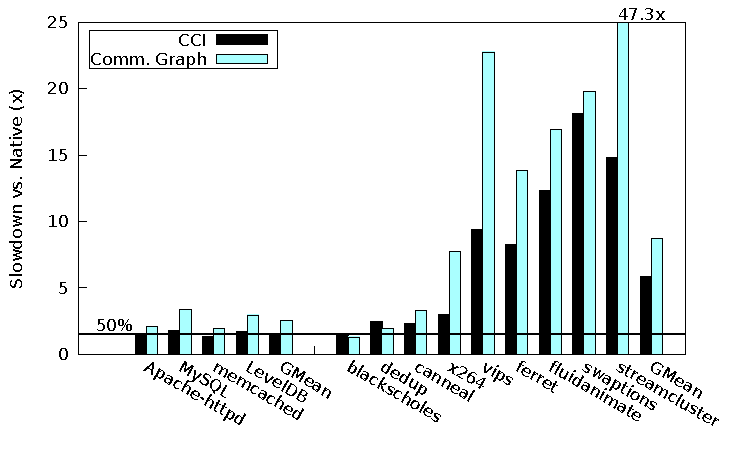
\includegraphics[width=.9\columnwidth]{plots/appperf.pdf}
\caption{\label{fig:perfapps}Performance overheads of CCI-Prev and Graph Collection implemented with \ctraps.}
\end{figure}


\subsection{Characterizing \ctraps}
\label{sec:char}
We characterized the instrumentation pruned by escape and redundancy analysis.
We report our results in Table~\ref{tab:char}.  Each column shows the percent
of instrumentation sites pruned and the absolute number of sites in
parenthesis.  The first column shows the amount of static instrumentation
pruned by escape analysis.  The second column shows the amount of static
instrumentation pruned by our redundancy analysis.  The third column shows how
many dynamic instances of instrumentation were eliminated by redundancy analysis.  To
collect the data in the third column, we implemented a special instrumentation
pass that marked pruned functions statically so they could be counted
separately from non-pruned functions at runtime.

\begin{table}
%\renewcommand{\tabcolsep}{2pt}
\centering
\small
\begin{tabular}{l | r r }
\multirow{3}{*}{\bf Application} & \multicolumn{2}{c}{\bf \em Pruned } \\
               & \multicolumn{2}{c}{\bf \em Static Local}  \\ 
               & \multicolumn{2}{c}{\bf \em Operations}    \\ \hline


Apache         &  21.4\%&(12K)                    \\
MySQL          &  21.3\%&(53K)                    \\
memcached      &  65.8\%&(7.5K)                   \\
LevelDB        &  44.0\%&(4.5K)                   \\ \hline
blackscholes   &   7.5\%&(4)                      \\
dedup          &   22.0\%&(171)                   \\
canneal        &   28.6\%&(226)                   \\
x264           &   29.8\%&(5960)                  \\
vips           &   24.6\%&(9116)                  \\
ferret         &   20.9\%&(792)                   \\
fluidanimate   &   19.6\%&(149)                   \\
streamcluster  &   11.6\%&(47)                    \\
swaptions      &   8.3\% &(19)                    \\
\end{tabular}
\caption{\label{tab:char}Instrumentation pruned by static analysis.}
\end{table}

The data show that escape analysis can prove a substantial fraction of
operations are local and do not require instrumentation.  Across PARSEC,
between 8\% and 30\% of accesses were proved local.  In the server programs, a
larger proportion of accesses were able to be proved local (21\% -- 66\%).  The
difference is likely due to the fact that server threads perform more
independent work (as discussed in Section~\ref{sec:eval:parsecserver}).  Eliminating
instrumentation using escape analysis is key to high performance.  

The data also show that fewer accesses were eliminated by redundancy analysis
than by escape analysis.  In some cases ({\em e.g.}, {\tt swaptions}), the
fraction of static and dynamic instrumentation sites eliminated is small.  In
these cases, the few pruned calls were infrequently executed and as
Figure~\ref{fig:perfapps} shows, there was little reduction in overhead.  In
other cases, like {\tt x264}, the fraction of calls pruned was substantial 
and yielded the largest performance boost.




\section{Related Work}

There are several categories of prior work related to last writer slices and \ctraps.  

\paragraph{Program Slicing}
Slicing techniques~\cite{tipslicingsurvey} are techniques for
identifying useful subsequences of a program's instructions.   Slicing can work
by analyzing program code statically or analyzing execution traces dynamically.
Many slicing techniques discussed in ~\cite{tipslicingsurvey} monitor control and
data dependences to identify which parts of a program might be relevant to a
task ({\em e.g., debugging}).

Thin Slicing~\cite{thinslicing} is related in its approach. Thin
Slicing monitors and reports a select subset of dependent operations from an
execution.  The goal is to eliminate some operations that would be included in a traditional
slice to make the slice simpler and less costly to collect.  While this work and
Thin Slicing differ in what they collect and how, our motivation to monitor a
select subset of dependences was similar to theirs.    Prior work
on slicing is unlike our work in that little has focused on monitoring
inter-thread dependences in production code without sampling or hardware support.

\paragraph{Communication Tracking in Concurrent Programs}
Several techniques have been proposed do some form of dependence and
communication tracking to analyze concurrent programs.  

CCI~\cite{cci}, Bugaboo~\cite{bugaboo}, Recon~\cite{recon}, and
DefUse~\cite{defuse} all explicitly track inter-thread memory dependences at
runtime.  Unlike our work, these techniques were not designed to run in
production systems~\cite{recon,defuse} without sampling~\cite{cci} or hardware
support~\cite{bugaboo}.  

Some other techniques~\cite{threadclustering,threadcriticality} have relied on
hardware debugging registers to monitor dependences efficiently enough for
production use.  These techniques are similar to our work in that they track how
threads interact ({\em i.e.}, share).  These techniques are different in that
their approach to dependence tracking is specific to the problem they address;
our system provides general support.

\paragraph{Extensible Program Instrumentation}
There are many systems for building analyses using extensible program
instrumentation.  Binary instrumentation
systems~\cite{pin,dynamorio,valgrind,roadrunner} provide completely general
support to instrument arbitrary code -- instrumenting a program to track
communciation is possible in such systems.  These systems are similar to
\ctraps in that they aim to enable dynamic analyses and runtime systems.  These
are different from \ctraps because they rely on dynamic rewriting, yielding
overheads too high for deployment.  \ctraps provides extensible support for a
restricted set of instrumentation tasks ({\em i.e.}, tracking communication)
with overheads low enough for production.  Such general systems also increase
the burden on implementors: to monitor communication, they must manually track
dependences, crafting delicate, performance sensitive code.  \ctraps tracks
only those dependences corresponding to communcation.  Furthermore, 
instrumentation systems lack the debugging benefits afforded by last writer slices.

\section{Conclusions}
This work stems from the observation that monitoring inter-thread communication
is often fast enough for use in deployed systems.  Based on this premise, we
develop system support for efficiently collecting last writer slices.  Using
that support, we developed \ctraps, a system for extensibly tracking
communicating inter-thread dependences.  \ctraps works efficiently at runtime,
in production, and without sampling or hardware support.  We showed that
\ctraps exposes a sound and complete (assuming race freedom) communication
tracking interface, enabling trap handlers to implement applications in just a
few lines of code.  We showed that a useful class of analyses can be
implemented using \ctraps that are efficient enough for deployment use in an
important set of programs ({\em e.g.}, servers, key-value stores, databases,
{\em etc.}).  We showed that last writer slices provide information that is
helpful for understanding concurrency errors with nearly no overhead.  Our
future work includes studying the generality of possible \ctraps applications
and the role of minimal hardware support for \ctraps.  We will also further study the
impact of provenance information on debugging in both sequential and concurrent
applications. 




\bibliography{bib}{}
\bibliographystyle{abbrv}

\end{document}
